% Intended LaTeX compiler: xelatex
\documentclass{orgstandard}
\author{ITT-Net-IS}
\date{\today}
\title{Einführung in den IT-Grundschutz des BSI\\\medskip
\large IT-Sicherheit}
\hypersetup{
 pdfauthor={ITT-Net-IS},
 pdftitle={Einführung in den IT-Grundschutz des BSI},
 pdfkeywords={},
 pdfsubject={},
 pdfcreator={Emacs 31.0.50 (Org mode 9.7.11)}, 
 pdflang={German}}
\begin{document}

\maketitle
\section{Das Bundesamt für Sicherheit in der Informationstechnik (BSI)}
\label{sec:org9ed000d}

\begin{center}
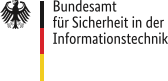
\includegraphics[width=1.5cm]{img/BSI_logo.png}
\end{center}

Das BSI ist die zentrale deutsche Cyber-Sicherheitsbehörde und fungiert als Gestalter der Informationssicherheit in Deutschland. Das BSI wurde 1991 gegründet und hat seinen Hauptsitz in Bonn.
Zu den Hauptaufgaben gehören:
\begin{itemize}
\item Entwicklung von Sicherheitsstandards und -richtlinien
\item Beratung von Behörden und Unternehmen in Sicherheitsfragen
\item Zertifizierung von IT-Produkten und Systemen
\item Aufklärung der Öffentlichkeit über IT-Sicherheitsrisiken
\item Abwehr von Cyberangriffen auf kritische Infrastrukturen
\end{itemize}
\section{Der IT-Grundschutz des BSI}
\label{sec:orgddaacab}

Der IT-Grundschutz bietet eine systematische Methodik zur Identifizierung und Umsetzung angemessener Sicherheitsmaßnahmen für IT-Systeme. Das \href{https://www.bsi.bund.de/DE/Themen/Unternehmen-und-Organisationen/Standards-und-Zertifizierung/IT-Grundschutz/IT-Grundschutz-Kompendium/it-grundschutz-kompendium\_node.html}{IT-Grundschutz-Kompendium} beschreibt praxisnahe Anforderungen und Maßnahmen für verschiedene IT-Komponenten und -Systeme.
\subsection{Die wesentlichen Schutzziele (CIA-Triade)}
\label{sec:org706d1a6}

\begin{center}
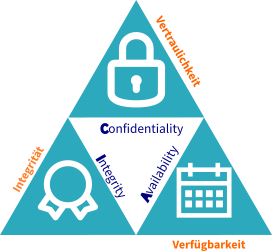
\includegraphics[width=.4\linewidth]{img/CIA.png}
\end{center}

Die drei grundlegenden Schutzziele der Informationssicherheit sind:
\begin{tolearn}
\begin{enumerate}
\item \textbf{Vertraulichkeit (Confidentiality)}: Informationen dürfen nur von autorisierten Personen eingesehen und bearbeitet werden.
\item \textbf{Integrität (Integrity)}: Die Korrektheit, Vollständigkeit und Unverfälschtheit von Informationen muss gewährleistet sein.
\item \textbf{Verfügbarkeit (Availability)}: Informationen und IT-Systeme müssen bei Bedarf funktionsfähig und zugänglich sein.
\end{enumerate}
\end{tolearn}
Ergänzende Schutzziele sind:
\begin{tolearn}
\begin{itemize}
\item \textbf{Authentizität}: Die Echtheit und Glaubwürdigkeit von Informationen und Identitäten.
\item \textbf{Nichtabstreitbarkeit}: Die Nachweisbarkeit von Handlungen und Transaktionen.
\item \textbf{Zurechenbarkeit}: Die eindeutige Zuordnung von Aktionen zu Personen oder Systemen.
\end{itemize}
\end{tolearn}
\section{Der IT-Grundschutz-Prozess}
\label{sec:org33f336b}

Der IT-Grundschutz-Prozess besteht aus folgenden Hauptphasen:
\begin{enumerate}
\item \textbf{Initiierung}: Einrichtung eines Informationssicherheitsmanagements
\item \textbf{Organisation}: Festlegung von Rollen, Verantwortlichkeiten und Ressourcen
\item \textbf{Strukturanalyse}: Erfassung aller relevanten Informationen, IT-Systeme und Geschäftsprozesse
\item \textbf{Schutzbedarfsfeststellung}: Bestimmung des Schutzbedarfs für jedes Objekt
\end{enumerate}
\begin{enumerate}
\setcounter{enumi}{4}
\item \textbf{Modellierung}: Abbildung der IT-Infrastruktur nach IT-Grundschutz
\item \textbf{IT-Grundschutz-Check}: Überprüfung der Umsetzung der Sicherheitsanforderungen
\item \textbf{Risikoanalyse}: Identifikation und Bewertung von Risiken
\item \textbf{Realisierung}: Umsetzung der Sicherheitsmaßnahmen
\item \textbf{Aufrechterhaltung}: Kontinuierliche Verbesserung
\end{enumerate}
\section{Beispielszenario: Mittelständisches Ingenieurbüro "TechPlan GmbH"}
\label{sec:orgab5ad95}


Die TechPlan GmbH ist ein Ingenieurbüro mit 50 Mitarbeitern, das Planungsleistungen für Industrieanlagen anbietet. Die IT-Infrastruktur umfasst:
\begin{itemize}
\item Einen Serverraum mit 5 physischen Servern
\item 50 Arbeitsplatzrechner
\item Ein internes WLAN und kabelgebundenes Netzwerk
\item Eine Internetverbindung mit Firewall
\item Spezielle CAD-Software für Konstruktionszeichnungen
\item Ein Dokumentenmanagementsystem für Projektdaten
\end{itemize}

Das Unternehmen arbeitet mit vertraulichen Kundendaten und wertvollen Konstruktionsplänen, die vor unbefugtem Zugriff geschützt werden müssen.
\subsection{Schritt 1: Initiierung des IT-Grundschutz-Prozesses}
\label{sec:org8731209}
Der Geschäftsführer hat die Bedeutung der Informationssicherheit erkannt und einen \textbf{IT-Sicherheitsbeauftragten} ernannt. Es wurde ein \textbf{Budget} für Sicherheitsmaßnahmen bereitgestellt.
\subsection{Schritt 2: Definition des Informationsverbunds}
\label{sec:org49a1d9c}
Der Informationsverbund wurde definiert als alle IT-Systeme, Anwendungen und Räumlichkeiten, die für die Geschäftsprozesse der TechPlan GmbH relevant sind.
\subsection{Schritt 3: Strukturanalyse}
\label{sec:org8c9dd6d}
In der Strukturanalyse wurden folgende \textbf{Komponenten} identifiziert:
\begin{itemize}
\item Geschäftsprozesse (Kundenakquise, Projektplanung, Konstruktion)
\item Anwendungen (CAD-Software, Dokumentenmanagementsystem, E-Mail)
\item IT-Systeme (Server, Arbeitsplatzrechner, Netzwerkkomponenten)
\item Räumlichkeiten (Serverraum, Büros)
\end{itemize}

\begin{NOTES}
CAD-Software (Computer-Aided Design) ist eine Software zur computergestützten Konstruktion, Modellierung und Detaillierung technischer Zeichnungen und 3D-Modelle in Bereichen wie Ingenieurwesen, Architektur und Produktdesign.
\end{NOTES}
\subsection{Schritt 4: Schutzbedarfsfeststellung}
\label{sec:org20ff01e}

Für jede Komponente wurde der Schutzbedarf nach den drei Grundwerten festgelegt:

\textbf{Beispiel: CAD-Daten und Konstruktionspläne}
\begin{itemize}
\item Vertraulichkeit: \textbf{HOCH} (Enthält wertvolles geistiges Eigentum)
\item Integrität: \textbf{HOCH} (Fehler können zu Planungs- und Produktionsfehlern führen)
\item Verfügbarkeit: \textbf{MITTEL} (Kurzzeitige Ausfälle sind verkraftbar)
\end{itemize}
\subsection{Schritt 5: Modellierung}
\label{sec:org1c9b1bc}
Die IT-Komponenten wurden den Bausteinen des IT-Grundschutz-Kompendiums zugeordnet:
\begin{figure}[!htpb]
\centering
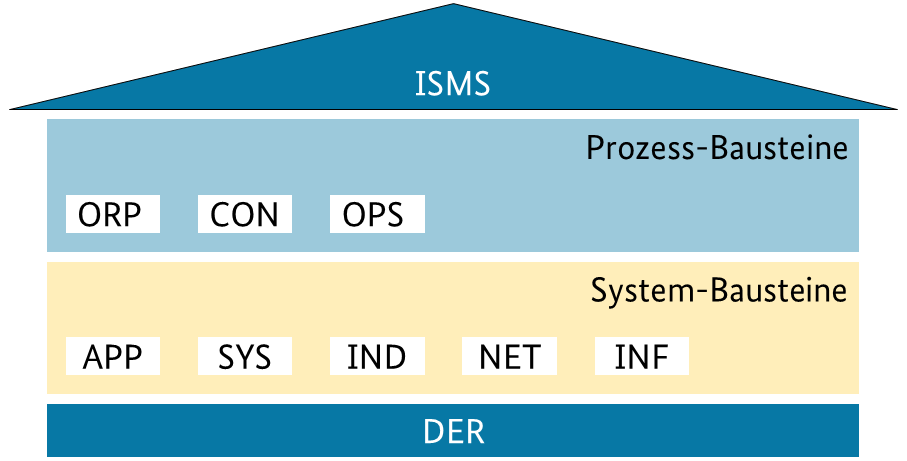
\includegraphics[width=.65\linewidth]{img/IT-Grundbausteine.png}
\caption{Bausteine IT-Grundschutz | Quelle: BSI-Kompendium}
\end{figure}
\begin{NOTES}
\begin{itemize}
\item \textbf{ISMS}: Sicherheitsmanagement
\item Prozessbausteine
\begin{itemize}
\item \textbf{ORP}: Organisation und Personal
\item \textbf{CON}: Konzepte und Vorgehensweisen
\item \textbf{OPS}: Betrieb
\end{itemize}
\item Systembausteine:
\begin{itemize}
\item \textbf{APP}: Anwendungen
\item \textbf{SYS}: IT-Systeme
\item \textbf{IND}: Industrielle IT
\item \textbf{NET}: Netze und Kommunikation
\item \textbf{INF}: Infrastruktur
\end{itemize}
\item \textbf{DER}: Detektion und Reaktion
\end{itemize}
\end{NOTES}
\section{Sicherheitskonzepte im Detail}
\label{sec:org64590b7}

IT-Sicherheit erfordert ein mehrschichtiges Konzept aus \textbf{technischen}, \textbf{organisatorischen} (TOM) sowie personellen \textbf{Maßnahmen}, das auf den IT-Grundschutz des BSI basiert und an die spezifischen Anforderungen einer Organisation angepasst werden muss.
\begin{NOTES}
Ein zentraler Aspekt ist die Verhältnismäßigkeit der Sicherheitsmaßnahmen im Verhältnis zum Schutzbedarf. Durch das Zusammenspiel dieser Maßnahmen entsteht eine mehrstufige Verteidigung nach dem Prinzip der \textbf{Defense-in-Depth}.
\end{NOTES}
\subsection{Zugangskontrolle (physischer Zugang)}
\label{sec:org2fe5f67}
\begin{itemize}
\item \textbf{Definition}: Maßnahmen, die den physischen Zugang zu IT-Systemen regeln.
\item \textbf{Beispiel bei TechPlan}:
\item Zutrittskontrollsystem mit Chipkarten für den Serverraum
\item Protokollierung aller Zutritte
\item Videoüberwachung an kritischen Zugangspunkten
\end{itemize}
\subsection{Zugriffskontrolle (logischer Zugriff)}
\label{sec:org60839ab}
\begin{itemize}
\item \textbf{Definition}: Maßnahmen, die den logischen Zugriff auf IT-Systeme und Daten regeln.
\item \textbf{Beispiel bei TechPlan}:
\item Rollenbasierte Zugriffsrechte im Dokumentenmanagementsystem
\item Zwei-Faktor-Authentifizierung für administrative Zugriffe
\item Berechtigungskonzept nach dem Need-to-Know-Prinzip
\end{itemize}
\subsection{Netzwerksicherheit}
\label{sec:org6d4883e}

Bei TechPlan wurden folgende Maßnahmen implementiert:
\begin{itemize}
\item Segmentierung des Netzwerks durch VLANs
\item Firewall mit restriktiven Regelsets
\item VPN für externen Zugriff
\item Intrusion Detection System zur Erkennung von Angriffsversuchen
\end{itemize}
\subsection{Datensicherung}
\label{sec:org0613bfe}

Die Datensicherungsstrategie umfasst:
\begin{itemize}
\item Tägliche inkrementelle Backups
\item Wöchentliche Vollsicherungen
\item Monatliche Auslagerung von Backup-Medien an einen externen Standort
\item Regelmäßige Tests der Wiederherstellbarkeit
\end{itemize}
\subsection{Notfallmanagement}
\label{sec:org572c7a9}

TechPlan hat ein Notfallkonzept erstellt, das folgende Aspekte umfasst:
\begin{itemize}
\item Notfallrollen und -verantwortlichkeiten
\item Eskalationswege
\item Wiederanlaufpläne für kritische Systeme
\item Jährliche Notfallübungen
\end{itemize}
\section{Praktische Umsetzung ausgewählter Maßnahmen}
\label{sec:org596ad7c}

Die theoretischen Sicherheitskonzepte müssen in der Praxis durch konkrete Maßnahmen umgesetzt werden. Diese Maßnahmen sind in drei Kategorien unterteilt:
\begin{enumerate}
\item Personelle Maßnahmen.
\item Technische Maßnahmen.
\item Organisatorische Maßnahmen.
\end{enumerate}

\begin{NOTES}
Diese Dreiteilung verdeutlicht den ganzheitlichen Ansatz des IT-Grundschutzes, der nicht nur auf technische Lösungen setzt, sondern auch die menschlichen und prozessualen Aspekte der Informationssicherheit berücksichtigt. 
\end{NOTES}
\subsection{Maßnahmen für Mitarbeiter}
\label{sec:orgd928c2f}
\begin{itemize}
\item Regelmäßige Sensibilisierungsschulungen
\item Klare Regelungen für den Umgang mit Passwörtern
\item Verpflichtung zur Einhaltung der Sicherheitsrichtlinien
\item Clean-Desk-Policy
\end{itemize}
\subsection{Technische Maßnahmen}
\label{sec:org565b9b9}
\begin{itemize}
\item Einsatz von Verschlüsselung für sensible Daten
\item Automatisierte Sicherheitsupdates
\item Zentrale Protokollierung und Auswertung von Sicherheitsereignissen
\item Malware-Schutz auf allen Systemen
\end{itemize}
\subsection{Organisatorische Maßnahmen}
\label{sec:orge3a5b25}
\begin{itemize}
\item Dokumentation der IT-Landschaft
\item Regelmäßige Sicherheitsaudits
\item Einbindung der Informationssicherheit in Veränderungsprozesse
\item Incident-Response-Prozesse
\end{itemize}
\end{document}
